%----------------------------------------------------------------------------------------
%	PACKAGES AND OTHER DOCUMENT CONFIGURATIONS
%----------------------------------------------------------------------------------------

\documentclass{article} % paper and 12pt font size
\usepackage{amsmath,amsfonts,amsthm} % Math packages
\usepackage[margin=1in]{geometry}
\usepackage[ruled,vlined]{algorithm2e}
\usepackage{graphicx}
\usepackage{float}
\usepackage[parfill]{parskip}
\usepackage[labelsep=quad,indention=10pt]{subfig}
\setlength{\paperwidth}{8.5in}
\setlength{\paperheight}{11in}

%----------------------------------------------------------------------------------------
%	TITLE SECTION
%----------------------------------------------------------------------------------------

\newcommand{\horrule}[1]{\rule{\linewidth}{#1}} % Create horizontal rule command with 1 argument of height

\title{	
\normalfont \normalsize 
\textsc{University of Texas at Austin, CS 391L} \\
\horrule{0.6pt} \\[0.4cm] % Thin top horizontal rule
\huge Homework 4 - Bayesian Network Approximate Inference \\[0.4cm]
\large Write Up  \\
\horrule{2pt} \\[0.5cm] % Thick bottom horizontal rule
}
\author{Venketaram Ramachandran\\
vr7948 - venket@cs.utexas.edu} % Your name
\date{\normalsize\today} % Today's date or a custom date

\begin{document}

\maketitle % Print the title

%----------------
% Approach
%----------------
\section{Overview}

In this assignment, I utilized Rejection Sampling as well as Gibbs Sampling to perform approximate inference on a hand-constructed Bayesian Network. As the assignment prompt requested, I constructed a simple Bayesian Network of 10 binary variables to perform inference. I specifically built the network such that it would not be a trivial network but simple enough to perform hand calculations to verify the results from approximate inference. Figure 1 shows the network that I created and used in this assignment, also containing the appropriate conditional probability tables for each node.

\begin{figure}[h]%
	\centering
    	\subfloat[]{%
        	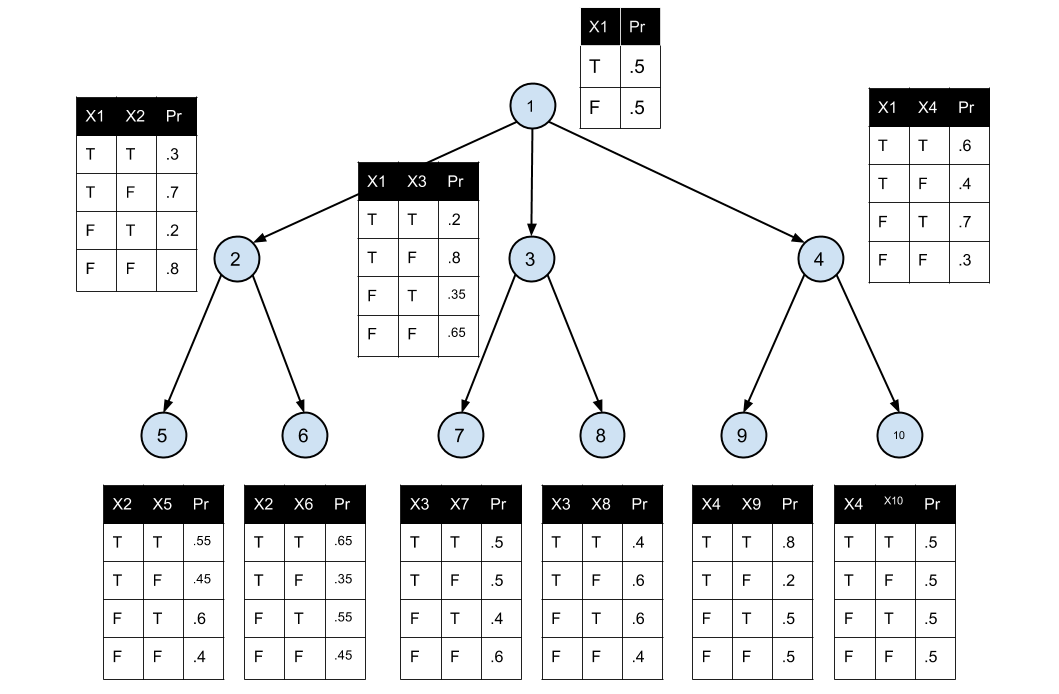
\includegraphics[width=120mm]{bayes_net_cpt.png}%
            \label{fig:left}%
        }\hfill%
    \caption{\textit{Bayes Net diagram and associated conditional probability tables}}
    \label{fig:default}
\end{figure}

The premise of the experiments was to answer conditional probability queries from the constructed Bayes Net through approximate inference techniques rather than exact inference. For the Bayes Net constructed and used in the assignment, though exact inference can be computed fairly easily, exact inference may not be as easy a task when the Bayes Net itself scales in other applications for non-toy examples. In the worst case, training, inference, or sampling, in particular, may become computationally intractable or at the very least extremely intensive. As a workaround, approximate inference techniques such as Gibbs Sampling or Rejection Sampling help provide an optimization in cost by providing a small tradeoff in accuracy. 

\subsection{Rejection Sampling}

For rejection sampling, the main idea is to first obtain a random sample for the data space according to the probability distributions. Then, if the values for the variables being conditioned in the query match that of the corresponding variables in the sample, the same is kept. Otherwise, the sample is rejected. The intuition here is that eventually enough samples will be accepted and since the accepted samples were taken according to the probability distributions in the data space, the frequency of the samples matching the values in query's variables will represent the approximate answer (i.e. probability value) for that query. At a large enough amount of accepted samples, the approximated answer should converge to the actual answer.

\subsection{Gibbs Sampling}

Gibbs Sampling is a Markov Chain Monte Carlo algorithm, similar to the Metropolis-Hastings algorithm from the previous Homework assignment in concept, in that it only uses the previous sample at each iteration to update each of the variables in the multivariate query, doing so one variable at a time. Gibbs sampling requires first an initialization point. Then, for each iteration, Gibbs sampling uses only the previous sample, clamped values, or variables already updated in the current iteration to incrementally update each non-clamped variable in the query. It does so by sampling a value for each variable conditioned on the other variables in the query, where the other variables take on their clamped value, their value from the update done in the current iteration if it exists, or the value from the previous sample (i.e. in that order). Though the Gibbs sample algorithm can start at an arbitrary point, the theory behind the sampling algorithm asserts that at a large enough number of iterations, the multivariate sample taken will approach the exact distribution for the query being answered.

\section{Approach}

In order to implement the Bayesian Network, I simply leveraged my own data structures and the Bernoulli function from the numpy Python library. Given my Bayesian Network, I could always simplify a lot of my queries. Therefore, I did not build a generic data structure for the Bayesian Network but rather simplified the overall joint distribution to the necessary distribution equations for each query and modeled those distributions in my code. This helped me create a fast implementation for Gibbs sampling and fast verification of the approximate inference.

My approach to implementing rejection sampling leveraged the ancestor sampling as mentioned in the homework prompt. For the sake of brevity, I will not repeat the approach mentioned in the prompt here. In regards to Gibbs sampling, the majority of work involved was in the conditional probability computation when resampling each component of the query, that was not already clamped, for the update rounds. However, my simplification of the distributions as referenced above helped make this segment efficient and I did not require any explicit data structures beyond that.

\section{Experiments}

\subsection{Setup}

Of the queries I ran when tinkering with my implementation and verifying its correctness, I have four that I officially used for experiments in order to demonstrate and identify differences between Gibbs and Rejection Sampling:

\begin{itemize}
\item \(P(X_1=T,X_5=F,X_9=T\ |\ X_3=T,X_4=F,X_2=T)\) - Selected since \(P(X_3=T,X_4=F,X_2=T)\) has a very small chance of being observed (i.e. 2.25\%).
\item \(P(X_2=T,X_2=T,X_4=T\ |\ X_1=T)\) - Selected since \(P(X_1=T)\) has a high chance (i.e. 50\%), relative to the other probabilities, of occurring.
\item \(P(X_4=T,X_6=F\ |\ X_1=T,X_3=F,X_2=T)\) - Less chance for the conditional being observed than \(P(X_1=T)\) but larger than \(P(X_3=T,X_4=F,X_2=T)\).
\item \(P(X_{10}=T,X_2=T\ |\ X_1=T,X_4=T)\) - Less chance for the conditional being observed than \(P(X_1=T)\) but larger than \(P(X_1=T,X_3=F,X_2=T)\).
\end{itemize}

Each query was run for one million iterations and all Gibbs sampling techniques used a burn-in of about 5\% of the total iterations. Literature mentions that there is no general way to exactly know the best burn-in rate so I went with a moderate, reasonable amount. Note that for rejection sampling, if a sample was thrown away at an iteration, I've counted it as staying at the same probability estimate so that it can be compared with Gibbs Sampling.

At one million iterations, both sampling techniques were well into convergence and, thus, I mainly saw a flat line for the overall curve. Therefore, the plot for the results did not provide much detail or insight. As a result, I reran the queries with less iterations (e.g. 50000 or 100000 iterations) to see patterns more clearly. 

\subsection{Results}

For completeness, Figure 2 below shows the results of the runs for 1000000 iterations. Figure 3 shows the results of the four queries after being run for a smaller number of iterations and the remainder of the results refers to that shown in Figure 3.

\begin{figure}%
	\centering
        \subfloat[Query 1]{%
        	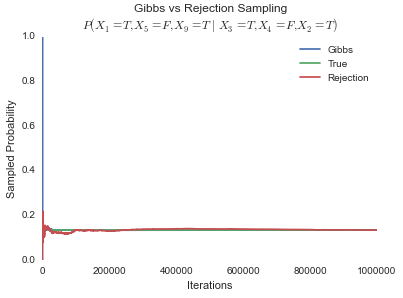
\includegraphics[width=70mm]{gr1_end.png}%
            \label{fig:left}%
        }\hfill%
        \subfloat[Query 3]{%
        	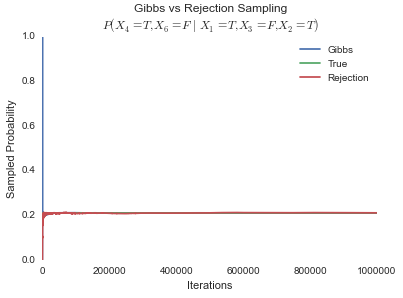
\includegraphics[width=70mm]{gr2_end.png}%
            \label{fig:right}%
        }\hfill%
        \subfloat[Query 2]{%
        	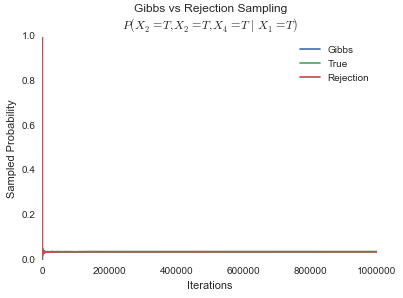
\includegraphics[width=70mm]{gr3_end.png}%
            \label{fig:right}%
        }\hfill%
        \subfloat[Query 4]{%
        	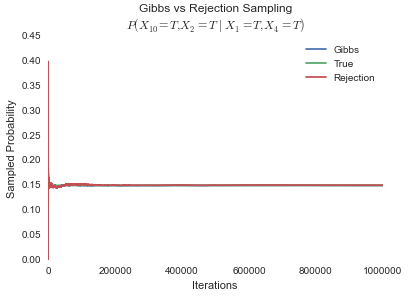
\includegraphics[width=70mm]{gr4_end.png}%
            \label{fig:right}%
        }
    \caption{\textit{Results of running the two sampling algorithms for one million iterations.}}
    \label{fig:default}
\end{figure}

\begin{figure}[h]%
	\centering
        \subfloat[Query 1]{%
        	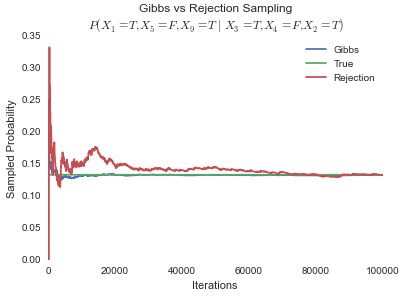
\includegraphics[width=70mm]{gr1.png}%
            \label{fig:left}%
        }\hfill%
        \subfloat[Query 3]{%
        	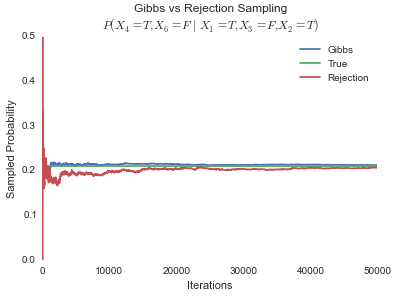
\includegraphics[width=70mm]{gr2.png}%
            \label{fig:right}%
        }\hfill%
        \subfloat[Query 2]{%
        	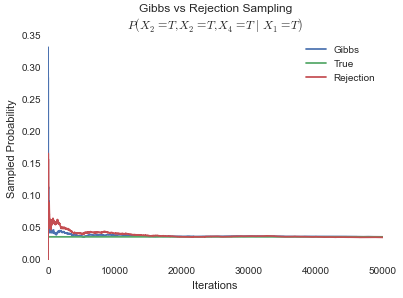
\includegraphics[width=70mm]{gr3.png}%
            \label{fig:right}%
        }\hfill%
        \subfloat[Query 4]{%
        	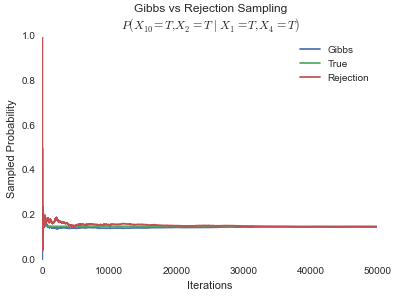
\includegraphics[width=70mm]{gr4.png}%
            \label{fig:right}%
        }
    \caption{\textit{Results of running the two sampling algorithms for fifty thousand or one hundred thousand iterations.}}
    \label{fig:default}
\end{figure}

It's clear that they converge well to the expected value but some interesting parts are prior to convergence. If we were to rank, in ascending order, the four queries based on the probability of observing their conditional, the ranking would be: Query 1, Query 3, Query 2, Query 4. I expected for this order to persist if we were to rank the results for Rejection Sampling by number of iterations to approach convergence, in descending order. From the results of the experiments, I can infer that my hypothesis was correct as visually inspecting the four graphs in Figure 3 confirms that notion. In general, this implies that rejection sampling is bound to throw away a lot more samples at higher dimensional spaces or for conditionals that have low probability of being observed.

On the other hand, note that in all four Queries, Gibbs sample does at least as good or much better, in terms of speed of convergence to the actual response, in comparison to Rejection Sampling. Again, both approaches converge at the limit. The speed at which they do, in terms of iterations, is the key point. 

The smallest margin of difference between the two sampling techniques occur in Queries 2 and 4, where the calculated probability of observing the conditional is .5 and .3 respectively. This implies that in these two cases Rejection Sampling threw away a lot less examples, relatively, and was able to converge faster. This is backed up by the results, where Rejection Sampling threw away 49.526\% and 69.99\% of the samples for Queries 2 and 4 respectively. Gibbs sampling is unaffected by this, as it performs essentially equally well in all four queries. Therefore, in these scenarios (i.e. 2 and 4), the overall convergence rate for both seem similar. However, in queries 1 and 3, where Rejection sampling rejects relatively more samples, Gibbs Sampling has a clear performance advantage. \\

In addition, note that due to the burn in, Gibbs Sampling does not have significant initial fluctuations and without I noticed some initial fluctuations. This makes sense since the point of burn in is to ignore the samples where the actual distribution not yet adequately enough captured by the Gibbs sampling technique. 

\section{Additional Discussion}

\subsection{Rejection Sampling Inefficiency}

Part of Rejection Sampling's inefficiency arises from the fact that it throws away so many examples whose values do not match that of the conditioned variables in the query. The amount of examples accepted corresponds directly to the probability of observing that series of values for the variables being conditioned on. For example, in Query 3, the probability of observing the condition \(X_1 = T\) is \(50\%\), which was reflected in the fact in that in the experiment 49.526\% of the samples were thrown away. Similarly, the probability of observing the condition \(X_2=T, X_3=T, X_4=F\) is approximately 2.25\%. For the corresponding query in Query 1, approximately 97.8\% of the samples were thrown away. 

It's easy to see how this can be a monumental problem as queries scale, queries become complex, or the dimensionality increases. If the probability of observing a particular condition is extremely tiny, rejection sampling will inefficiently throw away an immense number of examples, resulting in a great deal of wasted iterations. Furthermore, from this it can be seen that, in extremely high dimensional spaces, rejection sampling, as a result, becomes extremely unusable or at the very least unpalatable for usage, as the convergence will take significant resources. However, with that being said, Rejection Sampling still seems like a usable option in the context of much simpler queries (e.g. Query 2), where it does not become entirely sub-optimal in the face of complexity or high dimensionality. 

\subsection{Gibbs Sampling in Context of Random Sampling's Inefficiency}

Gibbs Sampling avoids the particular inefficiency problems discussed above for Random Sampling (i.e. this is not to say that Gibbs Sampling is perfectly efficient, it doesn't have that particular weakness found in Rejection Sampling). Gibbs Sampling does not try to randomly select-accept based on verifying a particular condition. Rather it tries to use the previous samples or clamps in conjunction with the conditional distributions present to obtain a new sample by resampling based on the probability of a particular variable, part of the multivariate query, conditioned on the other variables in the query. In this sense, intuitively, Gibbs Sampling aims to progressively to get closer and closer to the actual distribution at each sampling iteration.

From this perspective, it also intuitively makes sense why a burn in period is recommended for Gibbs Sampling. In the burn in period, the sampling algorithm throws away all samples but retains the last sample at each point to use for sampling in the next iteration. During that period, the burn in intuitively helps Gibbs start at a better approximation point for the true distribution. Given that the theory behind Gibbs Sampling asserts that it will continue to get closer to the true distribution, the amount of the burn in period can directly influence how many non-burn-in iterations it takes to converge.

\section{Future Work}

I would like to further explore burn in and thinning in context of Gibbs Sampling. Though I was able to tinker with the two when implementing Gibbs Sampling, due to time constraints, I was unable to properly include experiments regarding either in this report. Given that literature mentions that there isn't one particular surefire way to generate a best value for burn in or thinning, I would like to explore what qualities help decide a good burn in or thinning value and when in particular they provide the best boost.

Similarly, I found articles online regarding augmenting Rejection Sampling such as Adaptive Rejection Sampling. Given that Rejection Sampling has a seeming crippling flaw in high-dimensional spaces, I would like to see how best to still make use of it or understand what other scenarios can still make use of this tool, aside from cases such as Query 2.

\end{document}
